\section{Spielbeschreibung}

\begin{frame}
	\frametitle{Spielelemente und Aufgaben}
	\framesubtitle<1>{\textit{Tisch}}
	\framesubtitle<2>{\textit{Titanium Ores and Moon Rocks}}
	\framesubtitle<3>{\textit{Lunar Modules}}
	\framesubtitle<4>{\textit{Strategien}}

	\begin{figure}
		\begin{tikzpicture}
			\node[anchor=south west,inner sep=0] at (0,0) {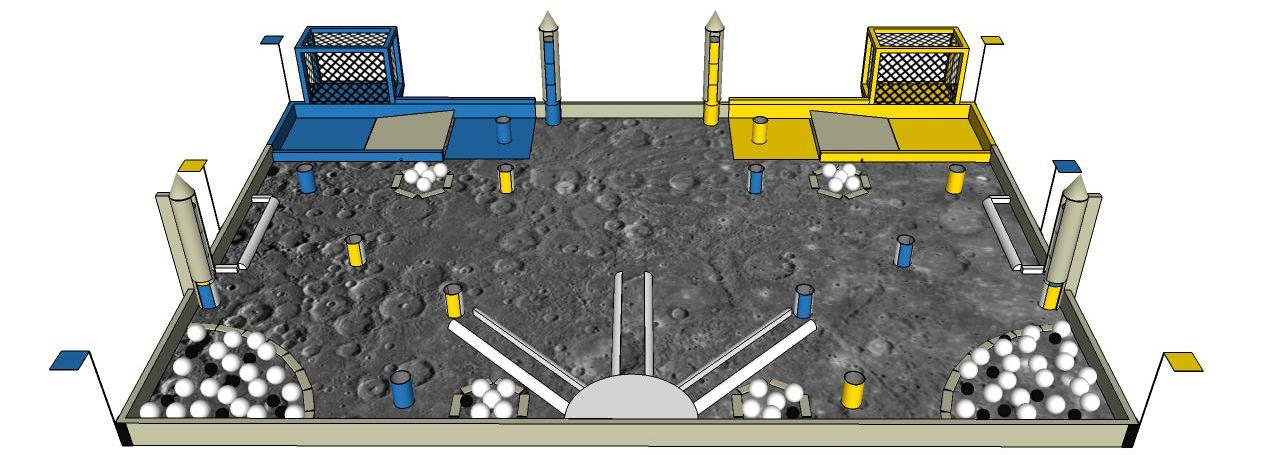
\includegraphics[width=13cm]{../images/presentation/spielfeldElemente.jpg}};
			\draw [draw=red, thick, visible on=<2>] (2.2,0.7) circle (0.9);
			\draw [draw=red, thick, visible on=<2>] (5,0.5) circle (0.4);
			\draw [draw=red, thick, visible on=<2>] (4.3,2.8) circle (0.3);
			\draw [draw=red, thick, visible on=<2>, ->] (3.5,2) -- (3.5,3.3);
			
			\draw [draw=red, thick, visible on=<3>] (1.5,1.3) rectangle (2.4,3);
			\draw [draw=red, thick, visible on=<3>] (5.4,3.3) rectangle (5.8,4.7);
			\draw [draw=red, thick, visible on=<3>] (10.4,1.3) rectangle (11.3,3);
			\draw [draw=red, thick, visible on=<3>] (3.1,2.8) circle (0.2);
			\draw [draw=red, thick, visible on=<3>] (5.2,2.8) circle (0.2);
			\draw [draw=red, thick, visible on=<3>] (3.6,2.1) circle (0.2);
			\draw [draw=red, thick, visible on=<3>] (4.6,1.6) circle (0.2);
			\draw [draw=red, thick, visible on=<3>] (4.1,0.7) circle (0.2);
			\draw [draw=red, thick, visible on=<3>] (7.7,2.8) circle (0.2);
			\draw [draw=red, thick, visible on=<3>] (9.2,2.1) circle (0.2);
			\draw [draw=red, thick, visible on=<3>] (8.2,1.6) circle (0.2);
			\draw [draw=red, thick, visible on=<3>, ->] (5.5,2.2) -- (6.5,1.2);
			\draw [draw=red, thick, visible on=<3>, ->] (5.5,2.2) -- (5.5,0.9);
			\draw [draw=red, thick, visible on=<3>, ->] (5.5,2.2) -- (7.9,1.2);
			\draw [draw=red, thick, visible on=<3>, ->] (2,3.3) -- (2.6,2.5);
			\draw [draw=red, thick, visible on=<3>, ->] (10.9,3.3) -- (10.2,2.5);
			
			\draw [draw=red, thick, visible on=<4>] (1.1,0) rectangle (5.8,4.7) node[pos=-0.05, shift={(2.6,0)}, color=red] {Arbeitsbereich grosser Roboter};
		\end{tikzpicture}
	\end{figure}
	
\end{frame}

\begin{frame}
	
	\frametitle{Wettbewerb}
	
	\begin{itemize}
		\item Homologation
	\end{itemize}
	\begin{itemize}
		\item 3 min Vorbereitungszeit
		\item 90 s Spiel
		\item \textit{Funny Action}
	\end{itemize}
	\begin{itemize}
		\item Finale \textit{Best-of-three}
	\end{itemize}
\end{frame}